\documentclass{report}
\usepackage{graphicx} % Required for \includegraphics
\usepackage{float}    % Required for [H] specifier

\begin{document}
\title{Labwork 6: Report}
\author{Nguyen Nhat Anh} % Required by the report class for \maketitle
\maketitle

\section{Introduction}
I have made the grayscale image binarization, brightness control, blending two images. All the code given are following strictly from report. 

\section{Results}
Image Binarization
\begin{figure}[H]
    \centering 
    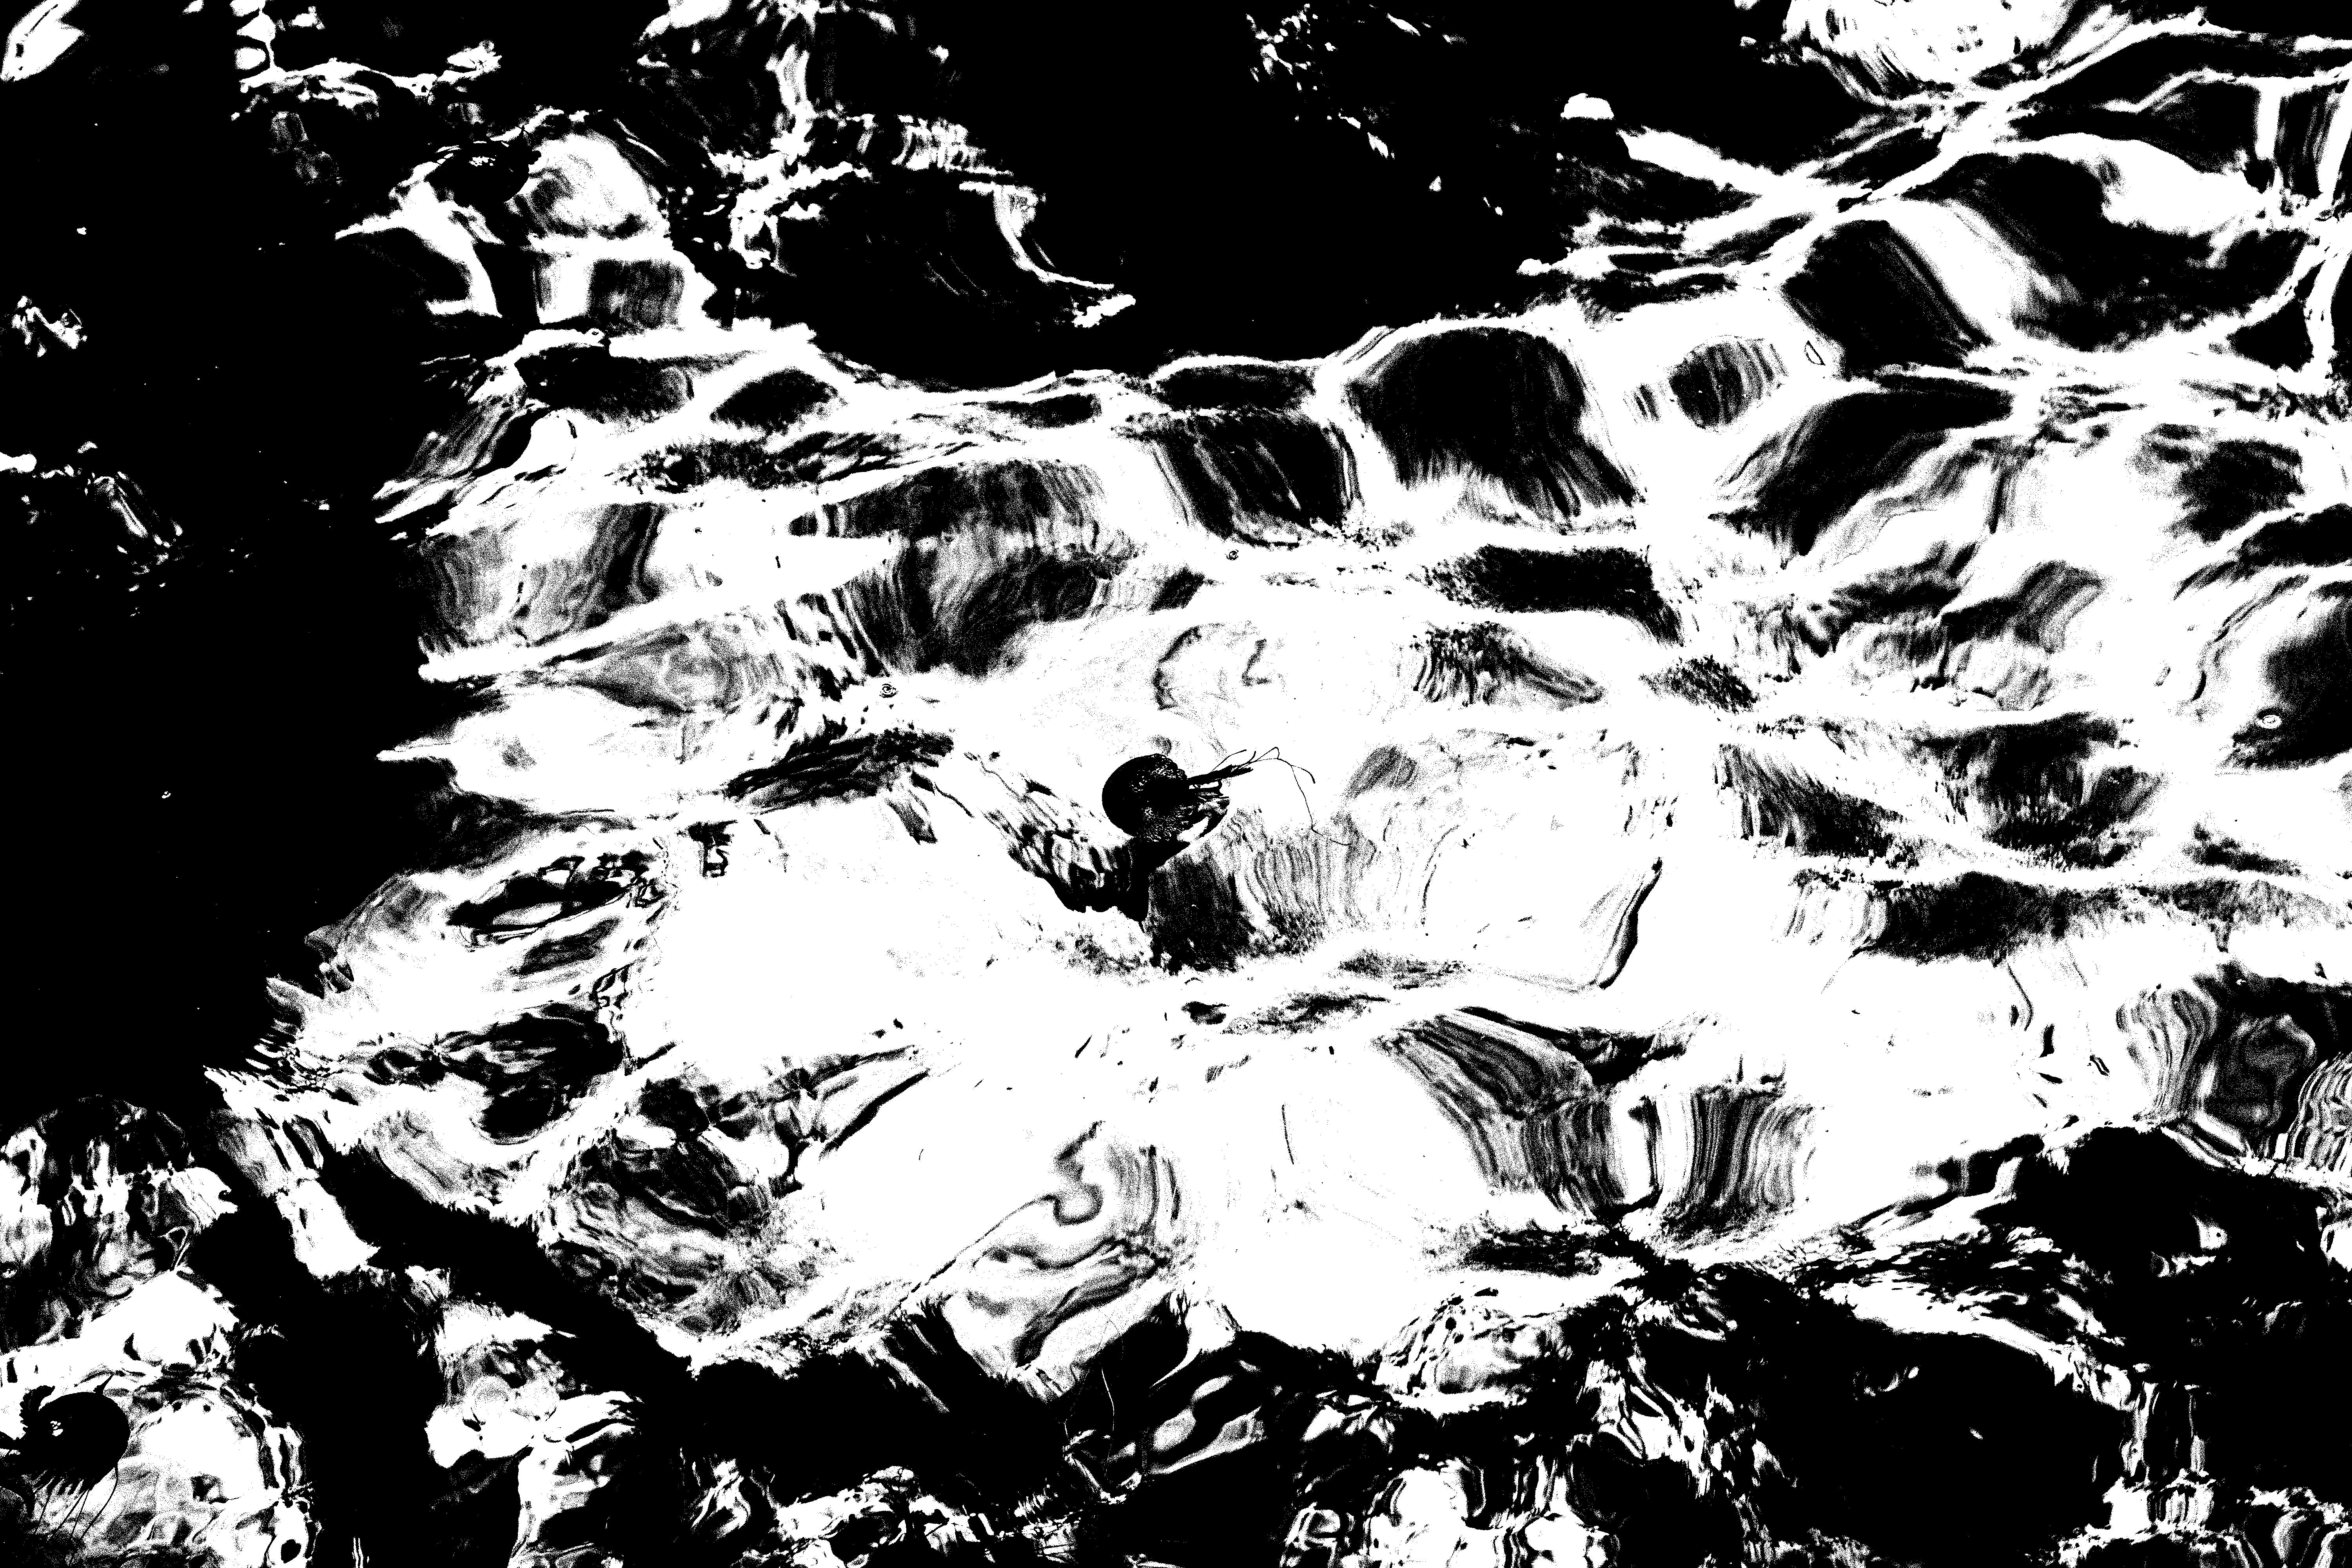
\includegraphics[width=0.7\linewidth]{output_binarized.jpg}
    \caption{Binarized Image.}
    \label{fig:binarized_img} 
\end{figure}

Image Brighness Control
\begin{figure}[H]
    \centering 
    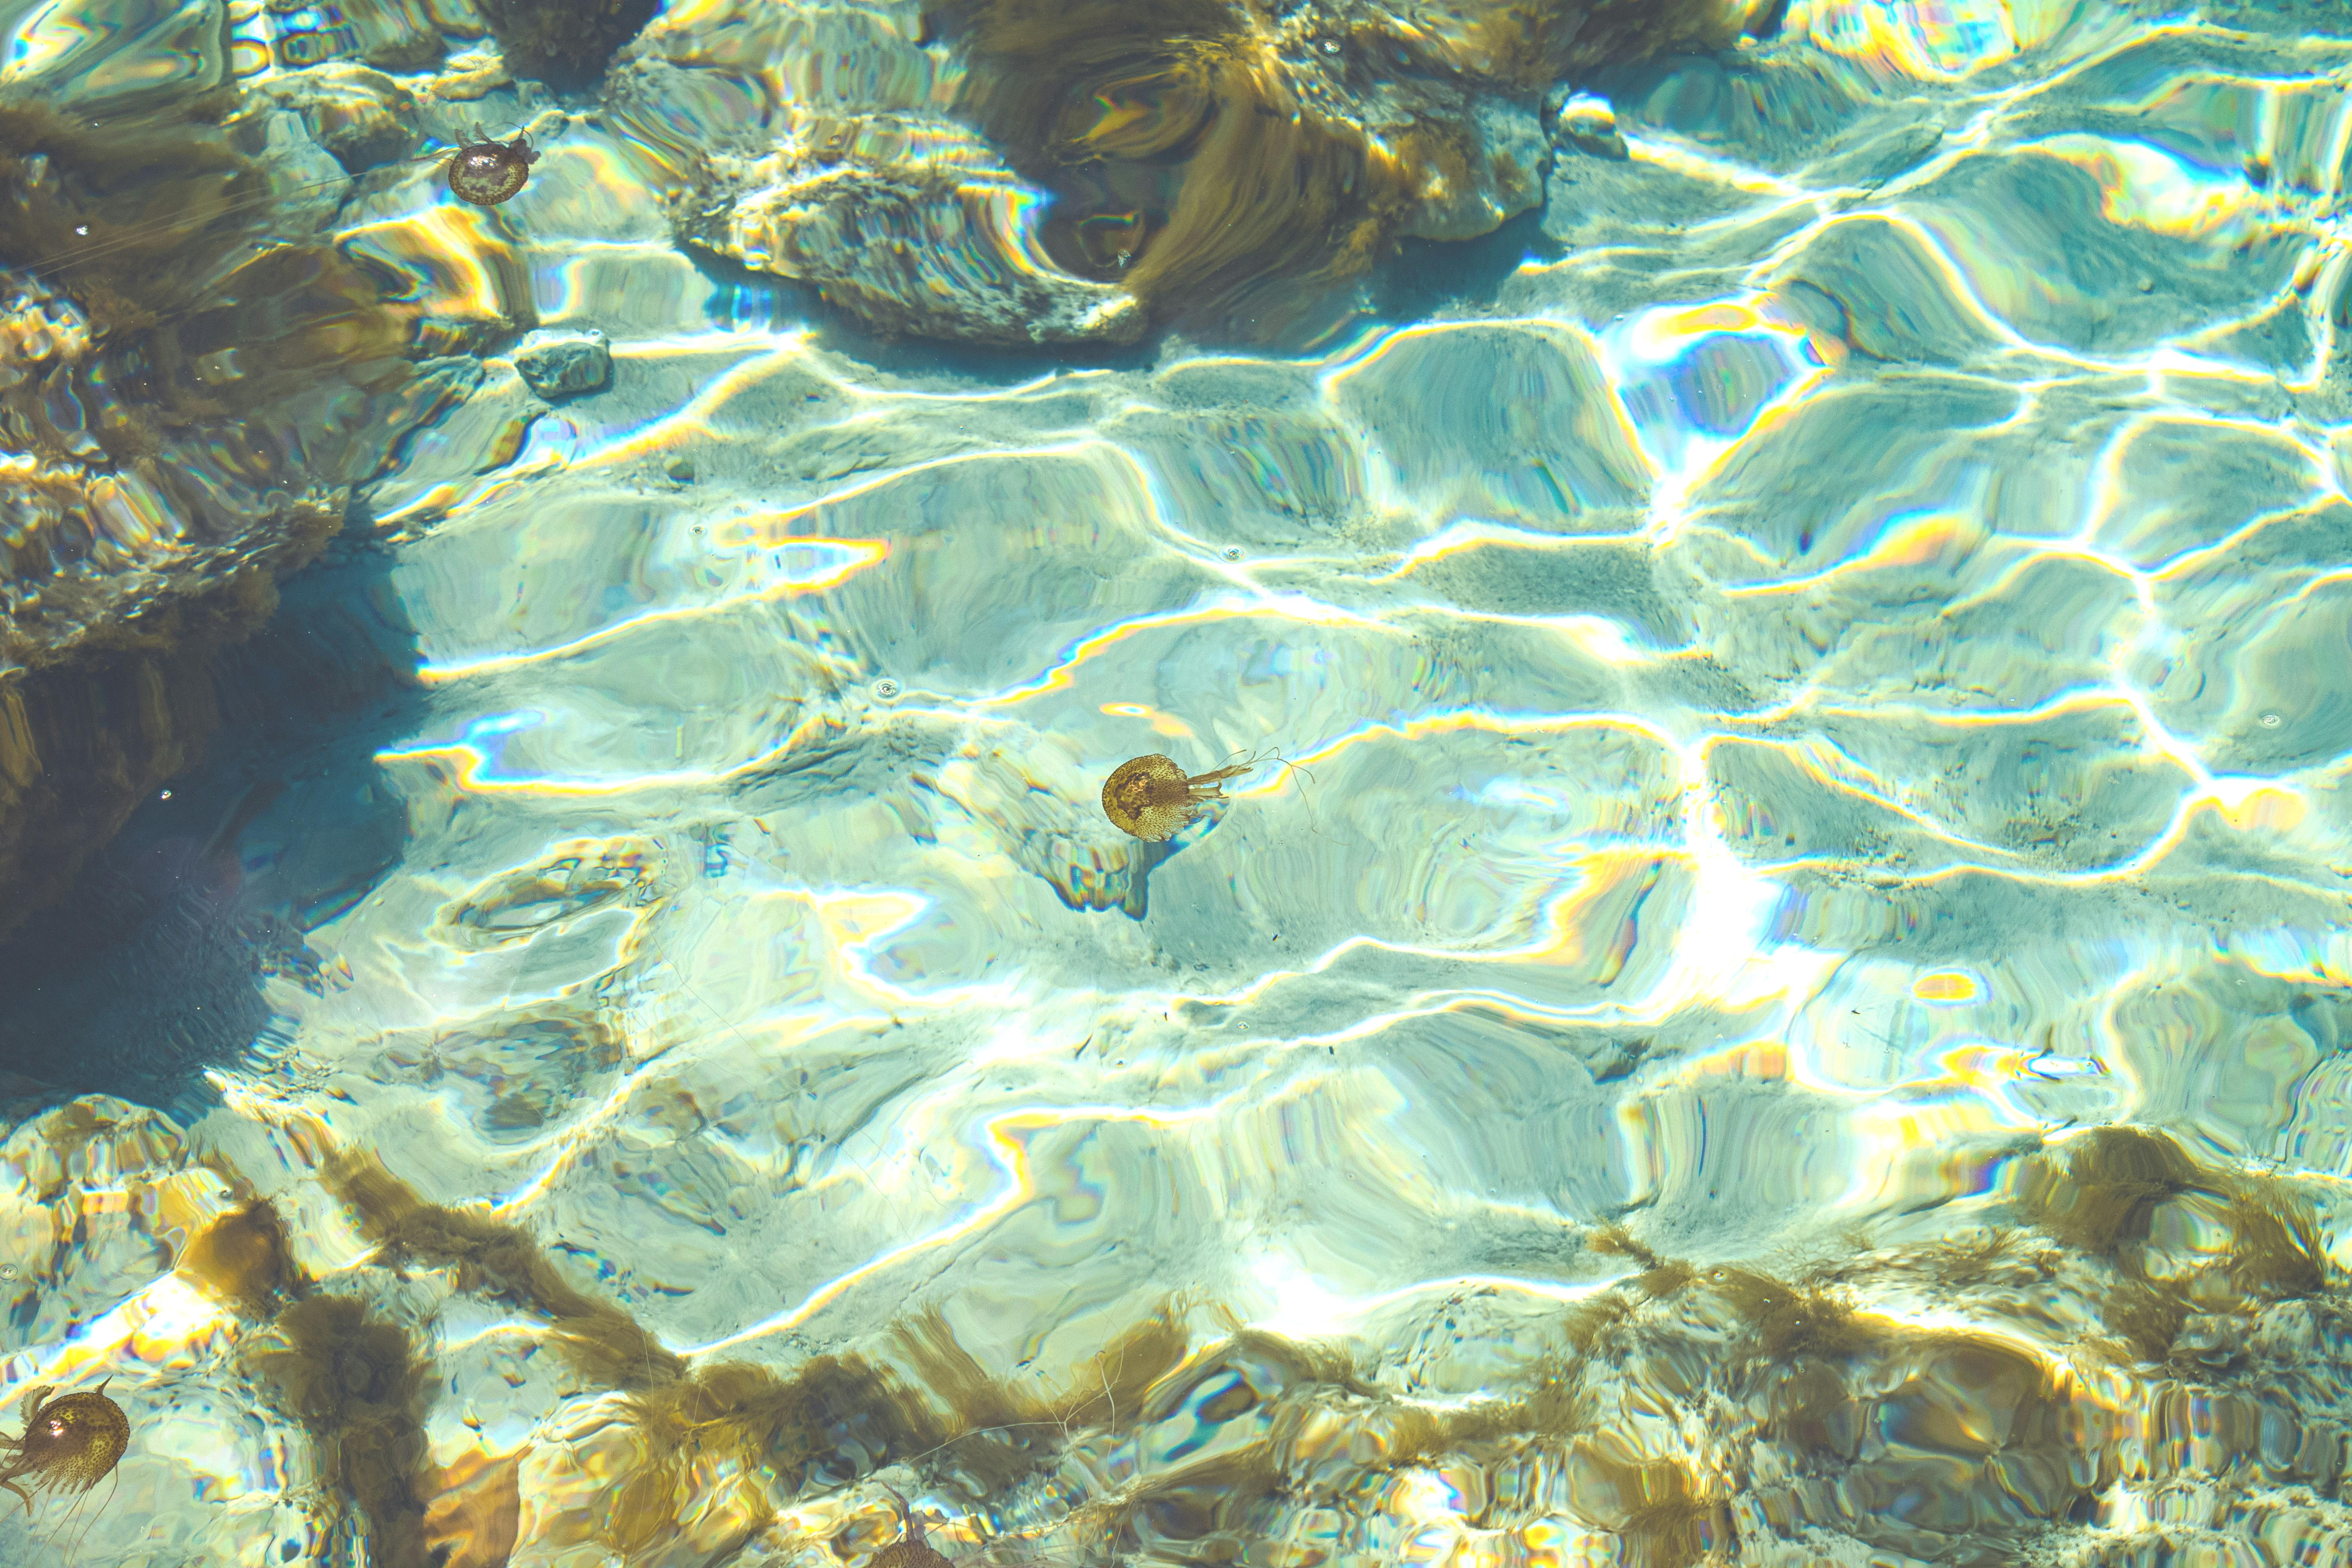
\includegraphics[width=0.7\linewidth]{output_brightness_inc.jpg}
    \caption{Inc. brightness Image.}
    \label{fig:image_inc}
\end{figure}

\begin{figure}[H]
    \centering 
    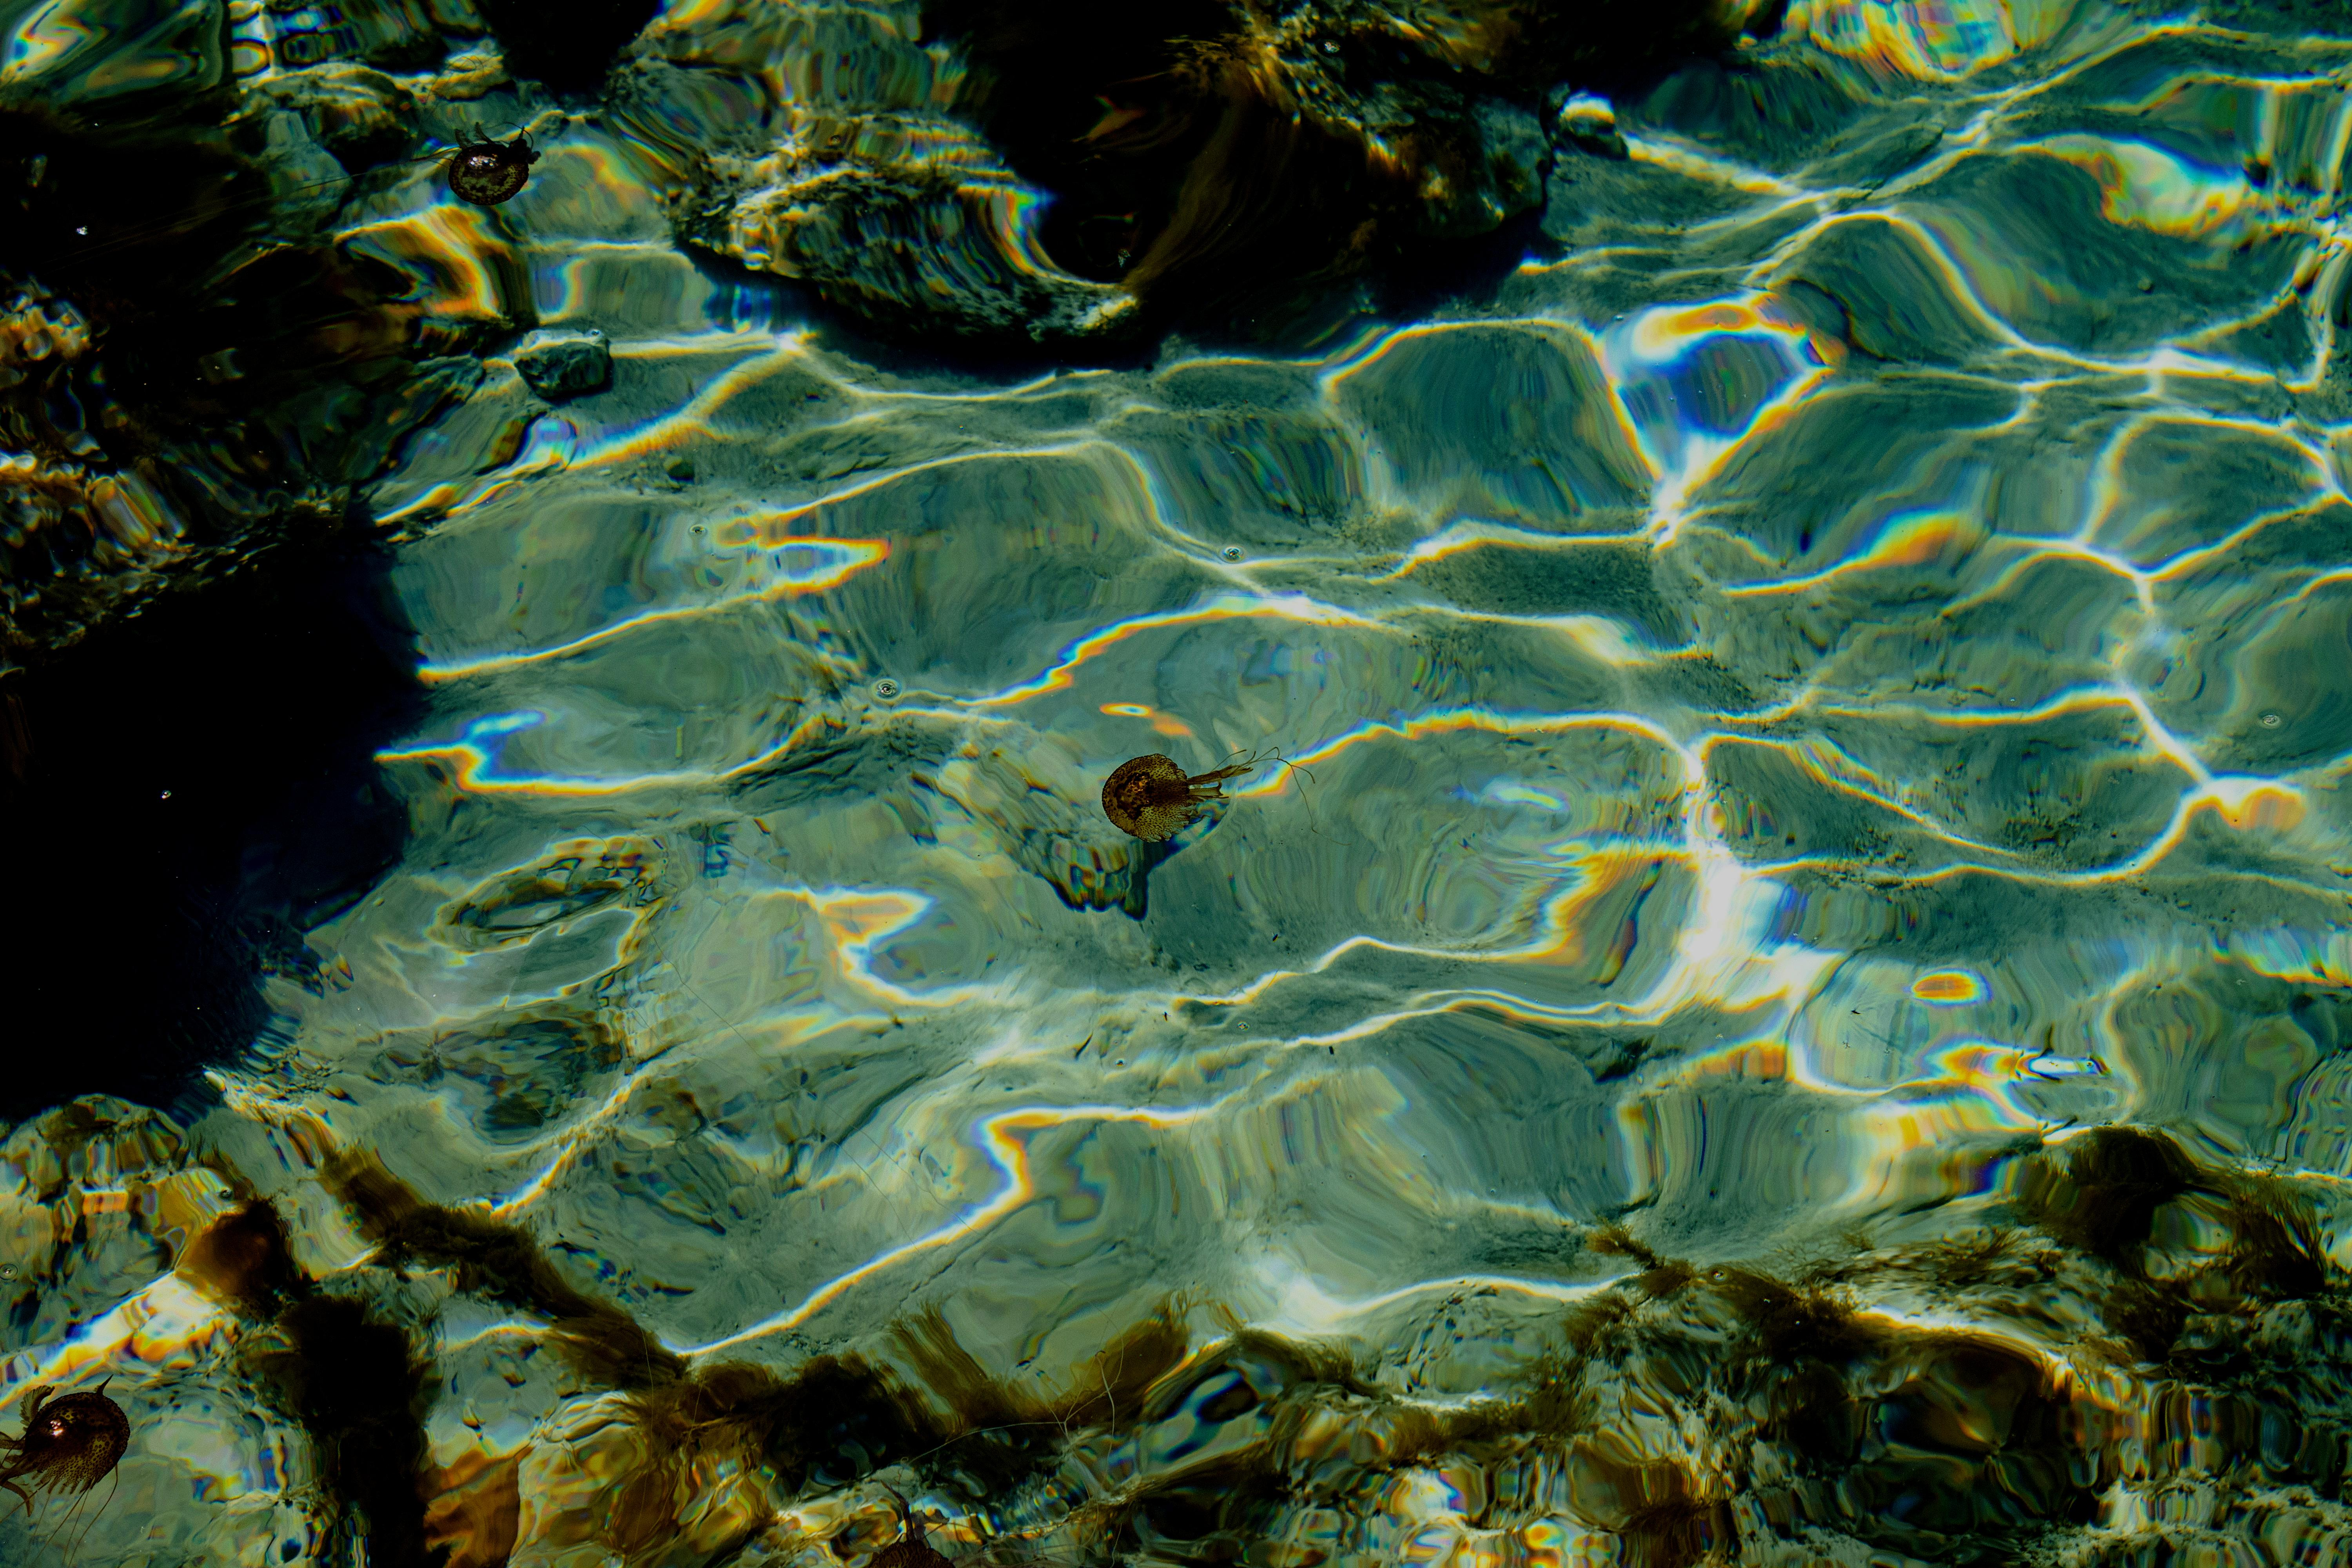
\includegraphics[width=0.7\linewidth]{output_brightness_dec.jpg}
    \caption{Dec. Brightness Image.}
    \label{fig:image_dec}
\end{figure}

Image blending
\begin{figure}[H]
    \centering 
    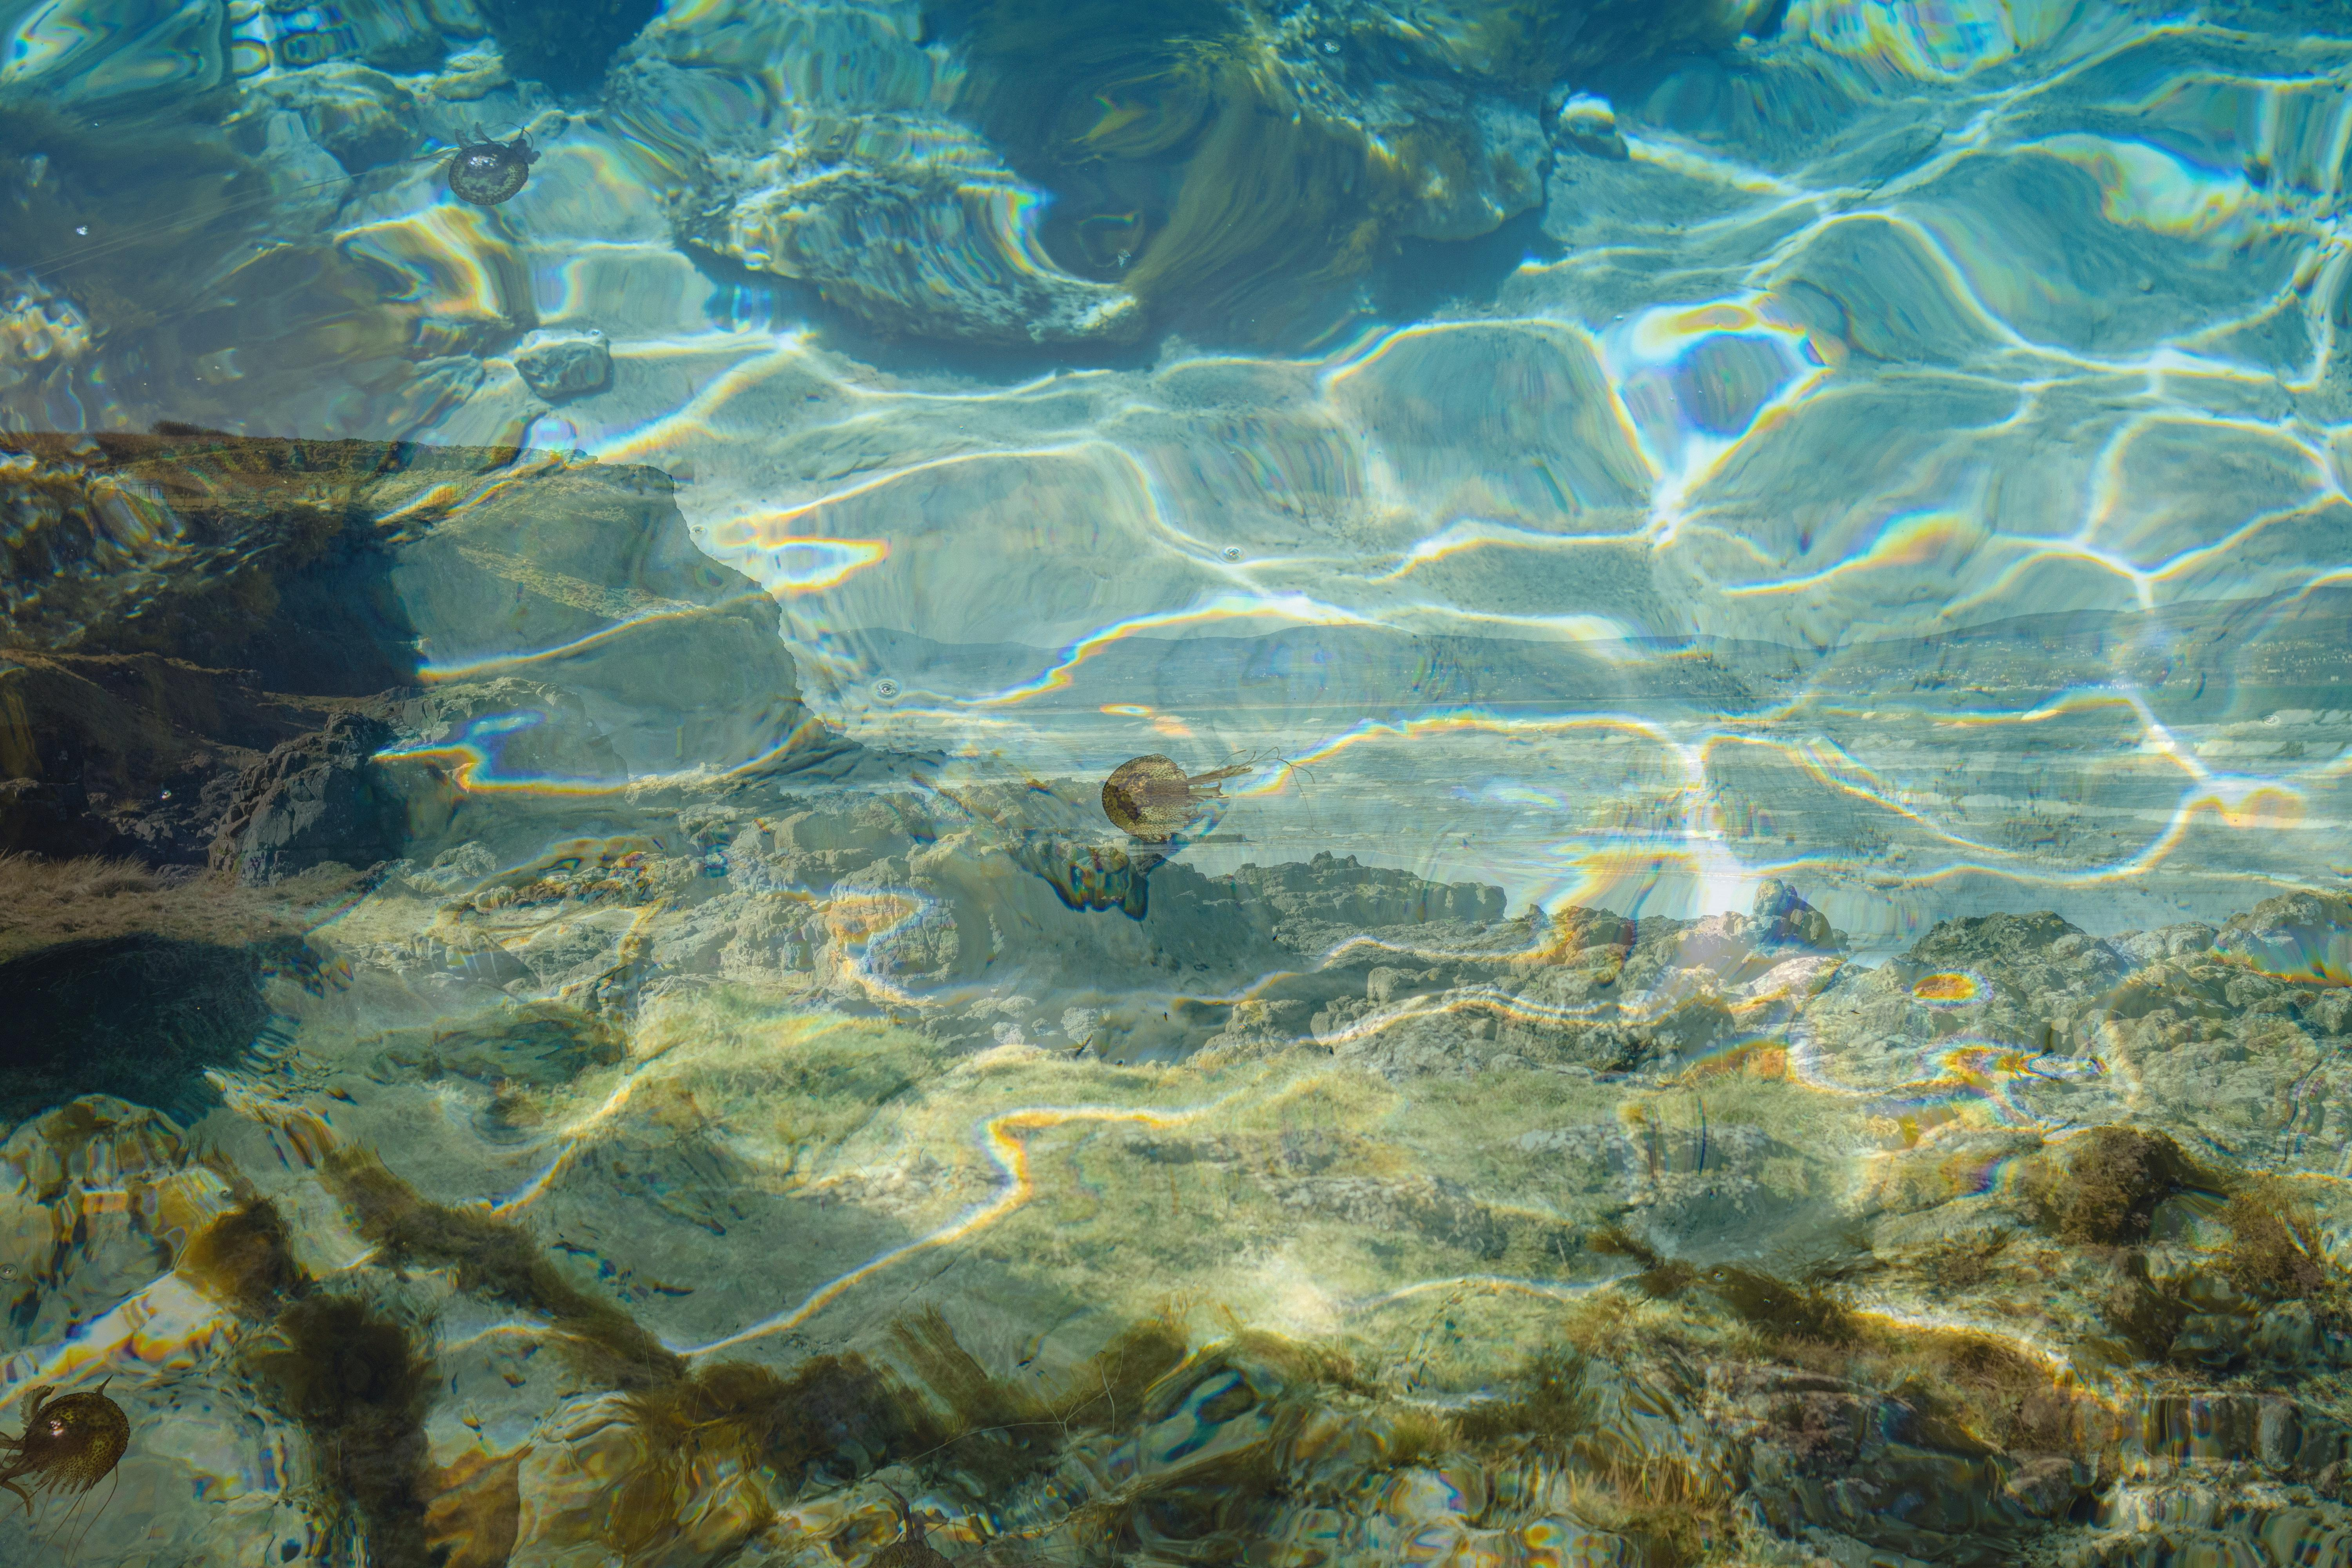
\includegraphics[width=0.7\linewidth]{output_blended.jpg}
    \caption{Image Blended.}
    \label{fig:blended_image}
\end{figure}

\section{Discussion}
The outputs show exacly expected outcomes from the labwork.
\end{document}